\documentclass{article}
\usepackage{amsmath}
\usepackage{amssymb}
\usepackage[a4paper, top=25mm, bottom=25mm, left=25mm, right=25mm]{geometry}
\usepackage{pgfplots}
\pgfplotsset{compat=1.18}
\usepackage{mathtools}
\DeclarePairedDelimiter\ceil{\lceil}{\rceil}
\DeclarePairedDelimiter\floor{\lfloor}{\rfloor}

\begin{document}
\pagestyle{empty}
\large

\begin{center}
2015-2016 Fall Semester\\MAT123-07 Midterm\\(10/12/2015)
\end{center}

\noindent 1. Find all local extrema and inflection points of the function $f(x)=\frac{1}{x}+\frac{1}{x^2}$. On which intervals is the function increasing, decreasing, concave upward, or concave downward? Find all asymptotes. Graph the function.


\hfill

\noindent 2. Use Rolle's theorem to show that $3\tan x + x^3 = 2$ has exactly one solution on the interval $[0,\pi/4]$.

\hfill

\noindent 3. Find the tangent line to the graph of the equation $x\sin\left(xy-y^2\right)=x^2-1$, at $(1,1)$.

\hfill

\noindent 4. Evaluate the limits.

\hfill

(a) $\displaystyle\lim_{x\to 0^+}(1+\sin x)^{\frac{1}{x}}$

(b) $\displaystyle\lim_{x\to 3}\frac{x^2-\floor{x^2}}{x-3}$

\hfill

\noindent 5. A point P is moving in the $xy$-plane. When P is at $(4, 3)$, its distance to the origin is increasing at a rate of $\sqrt{2}$ cm/s, and its distance to the point $(7, 0)$ is decreasing at a rate of 3 cm/s. Determine the rate of change of the $x$-coordinate of P at that moment.

\hfill

\noindent 6. Sketch the region bounded by $y=2|x|$ and $y=8-x^2$. Find the area of the region.

\newpage

\begin{center}
2015-2016 Fall Midterm (10/12/2015) Solutions\\
(Last update: 29/08/2025 20:34)
\end{center}

\noindent 1. Take the first derivative and set to 0.

\[f'(x)=-\frac{1}{x^2}-\frac{2}{x^3}\]
\[f'(x)=0\implies \frac{2}{x^3} = -\frac{1}{x^2}\implies x = -2 \quad(\text{candidate for a critical point})\]

\hfill

\noindent Take the second derivative and set to 0.

\[f''(x)=\frac{2}{x^3}+\frac{6}{x^4}\]
\[f''(x)=0\implies\frac{1}{x^3}=-\frac{3}{x^4}\implies x=-3\quad(\text{candidate for an inflection point})\]

\hfill

\noindent $\{-2,-3\}\subset\mathcal D$. Therefore, $f(-2)$ gives rise to a local extremum. The sign of the first derivative changes from minus to plus, meaning $f(-2)$ is a local minimum. $x=-3$ gives rise to an inflection point because the sign of the second derivative also changes.

\hfill

\noindent Find the asymptotes.

\[\lim_{x\to\infty}f(x)=\lim_{x\to-\infty}f(x)=0\]

\hfill

\noindent $y=0$ is the horizontal asymptote and $x=0$ is the vertical asymptote.

\hfill

\noindent Let us find monotonicity and concavity. If the sign of $f'(x)$ is minus, the function is decreasing on the corresponding interval; otherwise, increasing. If the sign of $f''(x)$ is minus, the graph of the function is concave downward; otherwise, concave upward.

\begin{center}
    \large
    \begin{tabular}{ |c| c c c c| } 
    \hline
        $x$ & $(-\infty, -3)$ & $(-3, -2)$ & $(-2, 0)$ &  $(0, \infty)$ \\
        \hline
        $f'$ sign & - & - & + & - \\
        \hline
        $f''$ sign & - & + & + & + \\
        \hline
    \end{tabular}
\end{center}

\hfill

\noindent Eventually, sketch the graph.

\begin{center}
\begin{tikzpicture}
  \begin{axis}[
    axis lines = center,
    xlabel = $x$,
    ylabel = $y$,
    domain=-3:-0.1,
    samples=200,
    ymin=-0.3, ymax=10,
    xmin=-5, xmax=5,
    restrict y to domain=-1:8,
    restrict x to domain=-5:5,
    legend pos=outer north east,
    clip=true,
    scale=1.2
  ]
  
  \node[blue] at (3,6) {$f(x) = \dfrac{1}{x} + \dfrac{1}{x^2}$};
  \addplot[blue, thick, domain=-5:-0.1] {1/x + 1/(x^2)};
  \addplot[blue, thick, domain=0.1:4.4] {1/x + 1/(x^2)};
  
  \draw[dashed, red] (axis cs:-5,0.05) -- (axis cs:5,0.05);
  \draw[dashed, red] (axis cs:0.05,-30) -- (axis cs:0.05,30);
  \end{axis}
\end{tikzpicture}
\end{center}

\hfill

\noindent 2. Let $f(x) = 3\tan x + x^3 -2$. $f$ is continuous on $[0, \pi/4]$ and differentiable on $(0, \pi/4)$. By IVT (Intermediate Value Theorem), there exists at least one point where $f(x) = 0$ because $f(0) = -2$ and $f(\pi/4) = 1 + (\pi/4)^3$. Assume that we have two roots on the interval, so at some point c, $f'(c) = 0$.

\[f'(x) = 3\sec^2x + 3x^2\implies  f'(c) = 3\sec^2c + 3c^2 = 0\implies \sec^2c =-c^2 \]

\hfill

\noindent Since $-c^2 \leq 0$ and $\sec ^2c > 0$, there is no $c$ that satisfies the equation. This contradicts our assumption that we have two roots on the interval. By Rolle's theorem, there is only one root on the interval $[0, \pi/4]$.

\hfill

\noindent 3. Implicitly differentiate both sides.

\[\frac{d}{dx}\left[x \sin\left(xy-y^2\right)\right] = \frac{d}{dx}\left(x^2-1\right) \]

\[1\cdot\sin\left(xy-y^2\right)+x\cdot\cos\left(xy-y^2\right)\cdot\left[\left(1\cdot y+x\frac{dy}{dx}\right)-2y\frac{dy}{dx}\right]=2x\]

\hfill

\noindent Rearrange the equation to solve for $\frac{dy}{dx}$ through a careful and rigorous attempt.

\[x\cdot\cos\left(xy-y^2\right)\cdot\left[\left(1\cdot y+x\frac{dy}{dx}\right)-2y\frac{dy}{dx}\right]=2x-\sin(xy-y^2)\]

\[y+\frac{dy}{dx}(x-2y)=\frac{2x-\sin\left(xy-y^2\right)}{x\cdot\cos\left(xy-y^2\right)}\]

\[\frac{dy}{dx}(x-2y)=\frac{2x-\sin\left(xy-y^2\right)}{x\cdot\cos\left(xy-y^2\right)}-y\]

\hfill

\begin{equation}\frac{dy}{dx}=\frac{\frac{2x-\sin(xy-y^2)}{x\cdot\cos(xy-y^2)}-y}{(x-2y)}\end{equation}

\hfill

\noindent Calculate $\left.\dfrac{dy}{dx}\right|_{(1,1)}$ from $(1)$. This will give us the slope of the tangent line.

\[\left.\frac{dy}{dx}\right|_{(1,1)}=-1\]

\hfill

\noindent Recall: $y-y_0 = m(x-x_0)$. $m$ is $\dfrac{dy}{dx}$ at $x=1$. So, the tangent line is:

\[y-1=-(x-1)\implies\boxed{y=2-x}\]

\hfill

\noindent 4.

\hfill

\noindent (a) Let L be the value of the limit. Then, take the logarithm of both sides.

\[L = \lim_{x\to 0^+} (1+\sin x)^{\frac{1}{x}}\]

\[\ln(L)=\ln\left[\lim_{x\to 0^+} (1+\sin x)^{\frac{1}{x}}\right]\]

\hfill

\noindent The expression on the right is continuous for $x>0$. Therefore, we can take the logarithm inside the limit.

\[\ln(L)=\lim_{x\to 0^+}\ln\left[(1+\sin x)^{\frac{1}{x}}\right]=\lim_{x\to 0^+}\left[\frac{\ln(1+\sin x)}{x}\right]\]

\hfill

\noindent If we substitute $x=0$, the limit is in the form $0/0$. L'Hôpital's rule states that we may take the derivatives of both sides of the fraction if there's a $0/0$ indeterminate form. Apply the chain rule accordingly.

\[\lim_{x\to 0^+} \left[\frac{\ln(1+\sin x)}{x}\right]\overset{\text{L'H.}}{=}\lim_{x\to 0^+} \left[\frac{\frac{1}{1+\sin x}\cdot\cos x}{1}\right]=\lim_{x\to 0^+}\left[\frac{\cos x}{1+\sin x}\right] \]

\hfill

\noindent The limit can now be evaluated by substituting $x=0$.

\[\lim_{x\to 0^+} \left[\frac{\cos x}{1+\sin x}\right] = \frac{\cos 0}{1 + \sin 0 } =1\]

\hfill

\noindent Now, $\ln(L) = 1$. Simply, take $L$ out of the logarithm.

\[ \boxed{L = \mathrm{e}}\]

\hfill

\noindent (b) Look at the one-sided limits. Let us first evaluate the limit from the right side. Above and near $x=3$, the floor function will return $9$.

\[ \lim_{x\to 3^+} \frac{x^2-\floor{x^2}}{x-3} = \lim_{x\to 3^+}\frac{x^2-9}{x-3} = \lim_{x\to 3^+}\frac{(x-3)(x+3)}{x-3} = \lim_{x\to 3^+}(x+3)= 6\]

\hfill

\noindent From the left side, the output is the largest integer less than $9$. Therefore, $\floor{x^2} = 8$.

\[ \lim_{x\to 3^-} \frac{x^2-\floor{x^2}}{x-3} = \lim_{x\to 3^-}\frac{x^2-8}{x-3} = -\infty\]

\hfill

\noindent The one-sided limits are not equal to each other. Therefore, the limit does not exist.

\hfill

\noindent 5. $x=x(t)$ and $y=y(t)$. The distance between the point P and the origin, and the distance between the point P and the point (7,0) are, respectively, given by:

\[f(t) = \sqrt{(x-0)^2 + (y-0)^2} = \sqrt{x^2+y^2}\]

\[g(t) = \sqrt{(x-7)^2 + (y-0)^2} = \sqrt{x^2-14x +49+y^2}\]

\hfill

\noindent Take the first derivative with respect to time.

\begin{equation}f'(t)=\frac{1}{2\sqrt{x^2+y^2}}\cdot\left(2x\frac{dx}{dt}+2y\frac{dy}{dt}\right)\end{equation}

\begin{equation}g'(t)=\frac{1}{2\sqrt{x^2-14x +49+y^2}}\cdot\left((2x-14)\frac{dx}{dt}+2y\frac{dy}{dt}\right)\end{equation}

\hfill

\noindent For $t=t_0$, it is given $x(t_0) = 4,\,y(t_0) = 3$ and $f(t_0) = \sqrt{4^2 +3^2} = 5,\,g(t_0) = \sqrt{3^2 + 3^2} = 3\sqrt{2}$. We then obtain a system of two equations by substituting values in (2) and (3):

\[f'(t_0)=\frac{1}{10}\cdot\left(8\frac{dx}{dt}+6\frac{dy}{dt}\right)=\sqrt{2}\]

\[g'(t_0)=\frac{1}{6\sqrt{2}}\cdot\left((-6)\frac{dx}{dt}+6\frac{dy}{dt}\right)=-3\]

\hfill

\noindent Let us simplify the equations.

\[4x'(t_0)+3y'(t_0) = 5\sqrt{2} \]
\[-3x'(t_0)+3y'(t_0) = -9\sqrt{2} \]

\hfill

\noindent The question asks us to find the change in the $x$-coordinate of P. Therefore, negate the latter equation and solve for $x'(t_0)$.

\[ \boxed{x'(t_0) = 2\sqrt{2}} \]

\hfill

\noindent 6.

\begin{center}
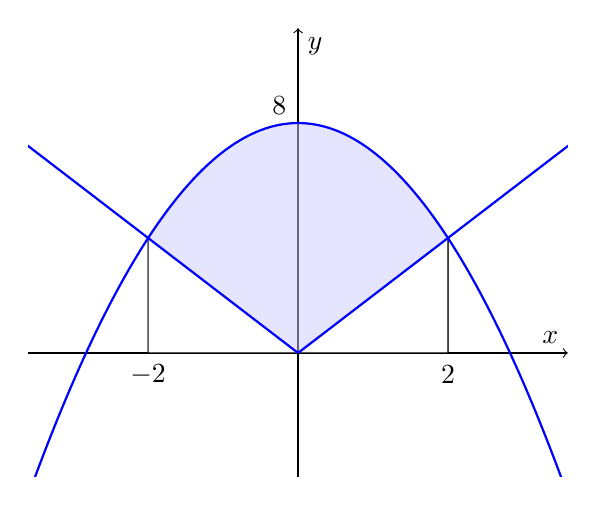
\begin{tikzpicture}
  \begin{axis}[
    axis lines = center,
    xlabel = $x$, ylabel = $y$,
    domain=-4:4,
    samples=300,
    ymin=-3, ymax=10,
    xmin=-3, xmax=3,
    restrict y to domain=-10:10,
    enlargelimits=true,
    legend pos=outer north east,
    axis line style={->},
    xtick=\empty, ytick=\empty
    ]
    \addplot [
      domain=-2:2,
      samples=200,
      fill=blue!20,
      opacity=0.5
    ]
    {8 - x^2} \closedcycle;

    \addplot [
      domain=-2:2,
      samples=200,
      fill=white,
    ]
    {2*abs(x)} \closedcycle;
    
    \addplot[blue, thick] {2*abs(x)};
    \addplot[blue, thick] {8-x^2};

    \node at (-2,-0.75) {$-2$}; \node at (2,-0.75) {$2$};
    \node at (-0.25,8.6) {$8$};

  \end{axis}
\end{tikzpicture}
\end{center}

\noindent The area can be found by integrating the difference in $y$ with respect to $x$. We split the integral into two because the absolute value function changes sign.

\[\mathrm{I}=\int_{-2}^2(8-x^2-2|x|)\,dx=\int_{-2}^0(8-x^2+2x)\,dx+\int_{0}^2(8-x^2-2x)\,dx\]

\[\mathrm{I}=\left[8x-\frac{x^3}{3}+x^2\right]_{-2}^0+\left[8x-\frac{x^3}{3}-x^2\right]_{0}^2\]

\[\mathrm{I}=0-\left({-16}+\frac{8}{3}+4\right)+\left(16-\frac{8}{3}-4\right)-0=\boxed{\frac{56}{3}}\]

\end{document}